\documentclass{beamer}

\mode<presentation>{
	%\usetheme{CambridgeUS}
	%\usecolortheme{seahorse}
	\usetheme{Boadilla}
	\usecolortheme{beaver}
	\setbeamertemplate{navigation symbols}{}
}

\usepackage{graphicx}
\usepackage{booktabs}
\usepackage{algpseudocode}
\usepackage{hyperref}
\usepackage{tikz}
\usepackage[utf8]{inputenc}
\usepackage{listings}
\usepackage[export]{adjustbox}
\usepackage{aeguill}

%\setbeamertemplate{title page}[default][rounded=false]

\setbeamertemplate{title page}
{
%\vbox{}
\begingroup
\centering
\begin{beamercolorbox}[sep=8pt,center]{institute}
\usebeamerfont{institute}\insertinstitute
\end{beamercolorbox}
\vskip1em%
\begin{beamercolorbox}[sep=8pt,center]{title}
\usebeamerfont{title}\inserttitle\par%
\ifx\insertsubtitle\@empty%
\else%
\vskip0.25em%
{\usebeamerfont{subtitle}\usebeamercolor[fg]{subtitle}\insertsubtitle\par}%
\fi%
\end{beamercolorbox}%
\vfill
\begin{beamercolorbox}[sep=8pt,center]{author}
\usebeamerfont{author}\insertauthor
\end{beamercolorbox}
\vskip1em\par
\begin{beamercolorbox}[sep=8pt,center]{date}
\usebeamerfont{date}\insertdate
\end{beamercolorbox}
\endgroup
}

\setbeamertemplate{blocks}[default]
\setbeamercolor{structure}{fg=darkred}
%\setbeamercolor{block title}{bg=darkred,fg=white}
%\setbeamercolor{block body}{bg=darkgray!20!white}
\setbeamercolor{block title}{bg=darkgray!30!white}
\setbeamertemplate{enumerate items}[default]

\setbeamertemplate{part page}{
\begin{beamercolorbox}[sep=8pt,center,wd=\textwidth]{part title}
\usebeamerfont{part title}\insertpart\par
\end{beamercolorbox}
\vfill
\tableofcontents
}

%\setbeamertemplate{frametitle continuation}{(\insertcontinuationcount)}

\setbeamertemplate{headline}{\leavevmode\hbox{\begin{beamercolorbox}[wd=.5\paperwidth,ht=2.65ex,dp=1.5ex,center]{section in head/foot}\usebeamerfont{section in head/foot}\insertsectionhead\hspace*{2ex}
\end{beamercolorbox}\begin{beamercolorbox}[wd=.5\paperwidth,ht=2.65ex,dp=1.5ex,center]{subsection in head/foot}\usebeamerfont{subsection in head/foot}\hspace*{2ex}\insertsubsectionhead\end{beamercolorbox}}\vskip0pt}

\setbeamertemplate{background}{\tikz[overlay,remember picture]\node[opacity=0.08]at (current page.south east){
\includegraphics[width=10cm]{figures/unibo_logo.jpg}};}

\newcommand{\tcc}[1]{\textcolor{darkred}{#1}}

\newcommand{\codeA}[1]{\texttt{#1}}
\newcommand{\codeB}[1]{\texttt{\textcolor{darkred}{#1}}}

\newcommand{\link}[1]{{\footnotesize » \url{#1}}}
\newcommand{\bothquote}[1]{``#1''}

\definecolor{mygreen}{rgb}{0,0.6,0}
\definecolor{mygray}{rgb}{0.5,0.5,0.5}
\definecolor{mymauve}{rgb}{0.58,0,0.82}
\definecolor{maroon}{rgb}{0.5,0,0}
\definecolor{darkgreen}{rgb}{0,0.5,0}

\lstset{
language=Java,
basicstyle=\scriptsize\ttfamily,
keywordstyle=\scriptsize\color{blue}\ttfamily,
commentstyle=\scriptsize\color{mygreen}\ttfamily,
breakatwhitespace=false,
breaklines=true,
 numbers=left,
  numberstyle=\color{mymauve},
  stringstyle=\color{mymauve},
  showstringspaces=false,
  numbers=none
}

\lstdefinelanguage{XML}
{
  basicstyle=\scriptsize\ttfamily,
  morestring=[s]{"}{"},
  morecomment=[s]{?}{?},
  morecomment=[s]{!--}{--},
  commentstyle=\color{darkgreen},
  moredelim=[s][\color{black}]{>}{<},
  moredelim=[s][\color{red}]{\ }{=},
  stringstyle=\color{blue},
  identifierstyle=\color{maroon},
  numbers=none
}

\makeatother

\AtBeginSection[]
{
  \begin{frame}
    \frametitle{Outline}
    \tableofcontents[currentsection]
  \end{frame}
}

%\AtBeginSubsection[]
%{
%  \begin{frame}
%    \frametitle{Outline}
%    \tableofcontents[currentsection,currentsubsection]
%  \end{frame}
%}

\institute[UNIBO]{\uppercase{Alma Mater Studiorum -- Università di Bologna}\\Dipartimento di Informatica -- Scienza e Ingegneria (DISI)\\C.d.S. in Ingegneria e Scienze Informatiche, Campus di Cesena}

\author[A. Marfoglia]{Alberto Marfoglia\\\scriptsize\texttt{alberto.marfoglia2@unibo.it}}


\title[Android -- 1C -- Background tasks]{Android programming}
\subtitle{Background Tasks}
\date[ver. 1.0 (20220505)]{Embedded Systems and Internet of Things\\A.A. 2021 -- 2022}

\begin{document}

\begin{frame}
  \titlepage
\end{frame}

\newcommand\blfootnote[1]{%
  \begingroup
  \renewcommand\thefootnote{}\footnote{#1}%
  \addtocounter{footnote}{-1}%
  \endgroup
}

\begin{frame}{Thanks}
    \centering
    \begin{itemize}
      \item \large{Professor Angelo Croatti}
    \end{itemize}

    \blfootnote{\url{https://www.unibo.it/sitoweb/a.croatti/en}}
    \blfootnote{}
\end{frame}

\section{Background tasks}

\begin{frame}{Background tasks}
  \begin{block}{Basics}
    All the components of an Android application are executed within the same
    process (\textit{Linux process}).
    \begin{itemize}
      \item It is created by the system during the startup of the first
      component.
    \end{itemize}
  \end{block}
  \begin{block}{"as long as possible" policy}
    \begin{itemize}
      \item Android ensures that each process is kept active for as much time as
      possible.
      \item \textbf{But} the system can decide to terminate the active process
      at any time.
    \end{itemize}
  \end{block}
\end{frame}

\section{The Main Thread}

\begin{frame}{The Main Thread (UI Thread)}
  \begin{block}{Fundamental}
    The Main thread is created when the application starts.
    \begin{itemize}
      \item All application's components are instantiated within it.
      \item It's responsible for managing all the events generated.
      \item \textbf{It's the only thread that can performs operations on the UI}. 
    \end{itemize}
  \end{block}
  \begin{block}{The Rule}
   In general, \textbf{you should take any blocking tasks off the UI thread}.
   \begin{itemize}
    \item In particular it cannot perform \textit{"long running tasks"}.
    \begin{itemize}
      \item Common tasks: accessing storage and performing network requests.
      \item The Android UI toolkit \textbf{is not thread-safe}.
    \end{itemize}
    \item If it gets stuck for more than 5 seconds, the system will shut down
    instantly the entire application.
   \end{itemize} 
  \end{block}
\end{frame}

\section{Worker Thread}

  \begin{frame}[fragile]{Worker Thread in action}
    \begin{block}{java.lang.Thread}
      In Android it is possible to take advantage of Java's support for
      Multi-Threading in order to create / execute new threads to perform
      long-running tasks.
    \end{block}
    \begin{exampleblock}{First attempt}
      \lstinputlisting[language=Java]{./code/1-background-task.java}
    \end{exampleblock}
  \end{frame}

  \begin{frame}[fragile,allowframebreaks]{Worker Thread in action -- Example}
   \begin{alertblock}{The problem}
    The previous code looks correct but ... \textbf{it doesn't work}
    \begin{itemize}
      \item It violates the principle that only tha Main thread can performs
      operations on the UI.
      \item Executing the \codeA{imageView.setImageBitmap(b)} statement in a
      thread different from the Main, will produce an exception at run-time.
    \end{itemize} 
   \end{alertblock}
   \begin{exampleblock}{The solution}
    The execution of the statement must be delegated to the Main thread.
    \begin{itemize}
      \item The \codeA{Activity} class provides: \codeB{runOnUiThread(Runnable
      action)}  
      \item If the method is performed by a different thread other than the
      Main, its execution will be queued in the \textit{Main Thread's event queue}.
    \end{itemize} 
   \end{exampleblock}

   \begin{exampleblock}{Second attempt}
      \lstinputlisting[language=Java]{./code/2-background-task.java}
   \end{exampleblock}

   \begin{block}{Considerations}
    \begin{itemize}
      \item In this case the code is thread-safe, but\dots
      \begin{itemize}
        \item Using multiple nested threads reduces the readability of the code 
      \end{itemize}
      \item To overcome this problem, Android provides two approaches:
      \begin{itemize}
        \item \tcc{Handler}: facilities the communication between the Worker and
        the Main thread.
        \item \tcc{AsyncTask}: It simplifies the execution of code, within a
        Worker, which affects the UI. 
      \end{itemize}
    \end{itemize} 
   \end{block}
  \end{frame}

\section{Handler}

  \begin{frame}{Handler}
    \begin{block}{Overview}
      A \codeA{Handler} allows you to send and process messages
      (\codeA{Runnable}) with a thread's message queue based on
      \tcc{MessageLoop} (\tcc{EventLoop}) pattern. 
      \begin{itemize}
        \item Generally used for communication between the Main thread and one or
        more Worker threads.
        \item When instantiated, the Handler is automatically bound to the control
        flow of the thread that creates it.
        \begin{itemize}
          \item If the handler is not instantiated within a MessageLoop, then
          you need to make it explicit.
        \end{itemize}
      \end{itemize}
    \end{block}
    \begin{block}{Remark}
      \begin{itemize}
        \item The Android Main Thread \textbf{is actually a MessageLoop}
      \end{itemize}
    \end{block}
  \end{frame}

  \begin{frame}{Handler - How it works}
    \begin{figure}
     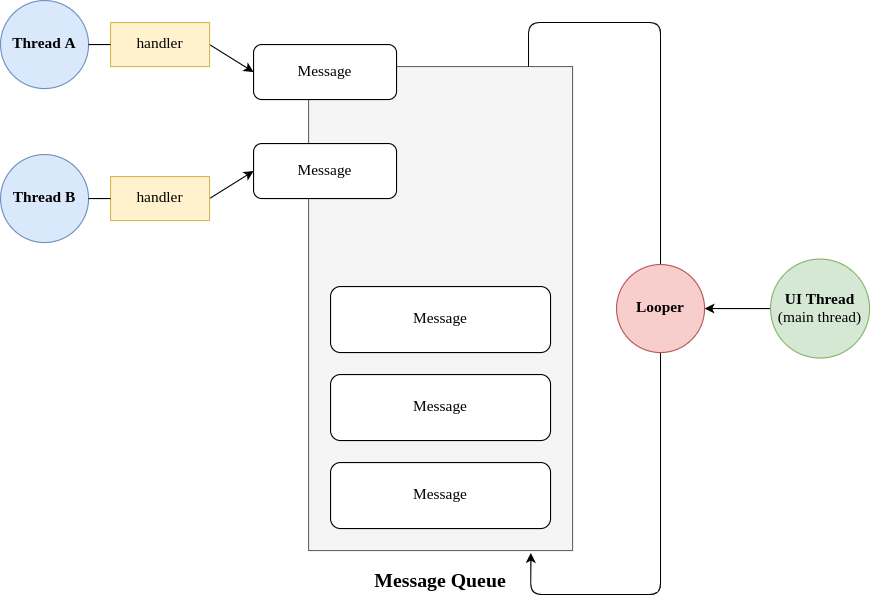
\includegraphics[width=0.85\textwidth]{figures/android-looper.png}
   \end{figure}
  \end{frame}

\subsection*{Example}

  \begin{frame}[fragile, allowframebreaks]{Handler -- Example} 
    \begin{exampleblock}{Handler for ImageDownloaderTask}
      \lstinputlisting[language=Java]{./code/1a-handler.java}
    \end{exampleblock}

    \begin{block}{General notes} 
      \begin{itemize}
        \item Each handler must extend from \texttt{android.os.Handler}
        \item The \codeA{handleMessage()} method allows you to intercept
        messages received by the handler and sent by the other threads.
        \item The \codeA{sendMessage()} method allows you to send a message to
        the handler.
        \begin{itemize}
          \item The message will be processed by the handler in the chosen
          Looper.
        \end{itemize}
      \end{itemize}
    \end{block}

    \begin{exampleblock}{Handler creation}
      \lstinputlisting[language=Java]{./code/1c-handler.java}
    \end{exampleblock}
  \end{frame}

  \begin{frame}{Example III}
    \begin{exampleblock}{Handler used by a WorkerThread}
      \lstinputlisting[language=Java]{./code/1b-handler.java}
    \end{exampleblock}
  \end{frame}

\subsection*{Message and Bundle}
  \begin{frame}{Message and Bundle}
    \begin{block}{Some notes}
      \begin{itemize}
        \item The transmitted message must be of type \codeB{Message}.
        \begin{itemize}
          \item The \tcc{what} field allows you to specify an integer value to
          discriminate the message received
          \item The are also other public fields to specify the content of the
          message \codeA{(arg1, arg2, obj, ...)}
        \end{itemize} 
        {\vspace{10pt}}
        \item To define the message's content it's better to use an object of type
        \codeB{Bundle}
        \begin{itemize}
          \item It defines the content according to the \codeA{key-value} pattern.
        \end{itemize}
      \end{itemize}
    \end{block}
  \end{frame}

\subsection{Android Looper}
  \begin{frame}[fragile]{Android Looper}
    \begin{block}{Overview}
      \begin{itemize}
        \item The \codeB{Looper.getMainLooper()} method allows you to retrieve
        the Main Thread's MessageLoop. 
        \item The \codeA{Looper} class allows to initialize any thread according
        to the MessageLoop pattern.
      \end{itemize}
    \end{block}

    \begin{exampleblock}{LooperThread -- Example}
      \lstinputlisting[language=Java]{./code/1d-handler-looper.java}
    \end{exampleblock}
  \end{frame}

\section{Async Task}

  \begin{frame}{Async Task}
    \begin{block}{Overview}
      \begin{itemize}
        \item An AsyncTask lets you to perform asynchronous computing on the UI
        \begin{itemize}
          \item Allows you to specify which portion of code should be run in
          background from a WorkerThread, and which one it should be delegated to
          the Main Thread.
          \item It doesn't require you to explicitly create the worker.
        \end{itemize}{\vspace{10pt}}
        \item It can be created by extending the \codeB{android.os.AsyncTask} class
        \begin{itemize}
          \item At least the \codeB{doInBackground()} method must be implemented,
          it contains the logic executed by the WorkerThread.
        \end{itemize}{\vspace{10pt}}
        \item It can be started by calling the \codeB{execute()} method on the
        instance.
      \end{itemize}
    \end{block}
  \end{frame}

  \begin{frame}[fragile]{Async Task -- Example}
    \begin{exampleblock}{ImageDownloader based on Async Task}
      \lstinputlisting[language=Java]{./code/1a-async-task.java}
    \end{exampleblock}
  \end{frame}

  \begin{frame}[allowframebreaks]{Async Task -- Details}
    \begin{block}{Callbacks}
      \begin{itemize}
        \item Four different methods can be redefined in an Async Task:
        \begin{itemize}
          \item \small{\codeB{onPreExecute()}, \codeB{doInBackground()},
          \codeB{onProgressUpdate()} and \codeB{onPostExecute()}}
        \end{itemize}
      \end{itemize}
    \end{block}

    \begin{block}{\codeA{void onPreExecute()}}
      \begin{itemize}
        \item It's invoked after the request for execution of the task itself. 
        \item It's execution is handled by the Main Thread.
        \item Generally used to setup the task.
      \end{itemize} 
    \end{block}
  \end{frame}

  \begin{frame}{Async Task -- Details II}
    \begin{block}{\codeA{Result doInBackground(Params... params)}}
      \begin{itemize}
        \item It's invoked immediately after \codeB{onPreExecute()} is terminated.
        \item It runs in a properly created worker thread.
        \item It receives as input the parameters passed to the \codeA{execute()}
        \item The result returned by the method is passed as input to the
        \item It can call the \codeA{publishProgress()} to perform minimal
        computation on the Main Thread \codeA{onPostExecute()} method.
      \end{itemize}
    \end{block}

    \begin{block}{\codeA{void onProgressUpdate(Progress... params)}}
      \begin{itemize}
        \item It's executed on the Main Thread whenever the
        \codeA{publishProgress()} method i called.
        \item It's receives the parameters passed to the \codeA{publishProgress} method.
      \end{itemize}
    \end{block}

  \end{frame}

  \begin{frame}{Async Task -- Details III}
    \begin{block}{\codeA{void onPostExecute(Result res)}}
      \begin{itemize}
        \item It's execute on the Main Thread following the termination of the
        \codeA{doInBackground()} method
        \item The result returned by \codeA{doInBackground()} is passed as an
        input parameter to the method. 
      \end{itemize}
    \end{block}
  \end{frame}
 
  \begin{frame}{Async Task -- Details V}
    \begin{block}{\codeA{AsyncTask<Params,Progress,Result>}}
      \begin{itemize}
        \item \codeB{AsyncTask<Params,Progress,Result>} is a parametric class
        that takes three parameters representing:
        \begin{itemize}
          \item \codeB{Params}: it is the type of the parameters that can be
          passed to the \codeA{doInBackground()} method.
          \item \codeB{Progress}: is the type of the parameters that can be passed
          to the \codeA{onProgressUpdate()} method. 
          \item \codeB{Result}: he is the return type of the \codeA{doInBackground()}
          method and therefore the input type of the \codeA{onPostExecute()} method.
        \end{itemize}
        \item These parameters can be specified with any type of data, including
        \codeB{Void} (no parameters).
      \end{itemize}
    \end{block}
  \end{frame}

  \begin{frame}[fragile,allowframebreaks]{Async Task -- Complete example}
    \begin{exampleblock}{ImageDownloader based on Async Task}
      \lstinputlisting[language=Java]{./code/1a-async-task-complete.java}
    \end{exampleblock}
    \begin{exampleblock}{}
      \lstinputlisting[language=Java]{./code/1b-async-task-complete.java}
    \end{exampleblock}
  \end{frame}

  \begin{frame}{Async Task Guidelines}
    \begin{block}{Guidelines}
      \begin{itemize}
        \item All the Async Task must be created in the Main Thread
        \begin{itemize}
          \item Only the Main Thread can call the \codeA{execute()} method on
          the instance of a task.
        \end{itemize}
        \item On each instance of Async Task, the \codeA{execute()} method can
        be called only once.
        \begin{itemize}
          \item Subsequent invocations throws an exception;
        \end{itemize}
        \item The 4 methods presented do not have to be called \textit{manually}
        on the task instance.
      \end{itemize}
    \end{block}
  \end{frame}


  \begin{frame}{Async Task -- Execution order}
    \begin{block}{Observations}
      \begin{itemize}
        \item \textbf{All the Async Task created and executed within the same application
        refer to the same WorkerThread}.  
        \begin{itemize}
          \item Eg: \small{If two async tasks are performed within the same
          application, the \codeA{doInBackground()} method of the second can be
          executed only after the termination of the same method of the first
          task.}
        \end{itemize}
        \item So you have to pay attention to the (potentially blocking) tasks
        that have to be performed in the \codeA{doInBackground()} method.  
      \end{itemize}
    \end{block}
    \begin{block}{Alternatives}
      If there's a need to perform tasks in parallel, there are other
      mechanisms:
      \begin{itemize}
        \item Run the task by calling the \codeB{executeOnExecutor()} function
        instead of the \codeA{execute()} method, specifying the \textit{executor}.
        \item Use the \tcc{Service} component.
      \end{itemize}
    \end{block}
  \end{frame}

  \begin{frame}{Async Task -- Last notes}
    \begin{block}{}
      AsyncTask is deprecated in API level 30, the officially recommended alternative 
      is \textbf{Kotlin Coroutines}\footnote{For details: \href{https://developer.android.com/topic/libraries/architecture/coroutines}{developer.android.com/coroutines}}.
      \begin{itemize}
        \item An unofficial alternative is to combine \codeB{java.util.concurrent.Executors} class with the \codeA{Handler}.
      \end{itemize}
    \end{block}
    \begin{exampleblock}{}
      \lstinputlisting[language=Java]{./code/1c-async-task-executor.java}
    \end{exampleblock}
  \end{frame}

\section*{Summary}
  \begin{frame}{Summary}
    \begin{block}{Comparison}
      \begin{itemize}
        \item \tcc{Handler}: you should use it if you are on an \textbf{non-UI thread},
        and you want to do something with UI.
        \item \tcc{runOnUiThread}: is a special case of more generic \texttt{Handlers}.
        \begin{itemize}
          \item if we are in a UI thread the runnable is executed immediately. 
          Otherwise, it will post it to the \texttt{Handler}.
          \item it may reduce the readability of the code.
        \end{itemize}
        \item \tcc{AsyncTask}: you should use it when you are on the \textbf{UI Thread} and you want 
        to run a long-running task (e.g. call a web service).
      \end{itemize}
    \end{block}
  \end{frame}



\section*{References}
%-----------------------
%--- ONLINE RESURCES ---
%-----------------------

\begin{frame}{References - Online Resources}
\begin{thebibliography}{99}
\setbeamertemplate{bibliography item}[online]

\bibitem{adAPIguide} Android Developers - Guide
\newblock \link{https://developer.android.com/guide/}

\bibitem{adAPIreference} Android Developers - API Reference
\newblock \link{https://developer.android.com/reference/}

\bibitem{adTraining} Android Developers - Samples
\newblock \link{https://developer.android.com/samples/}

\bibitem{adTraining} Android Developers - Design \& Quality
\newblock \link{https://developer.android.com/design/}

\end{thebibliography}
\end{frame}

%-----------------------
%--- BOOKS -------------
%-----------------------

%\begin{frame}{Riferimenti - Libri}
%\begin{thebibliography}{99}
%\setbeamertemplate{bibliography item}[book]
%
%\bibitem{Mednieks11} Zigurd Mednieks, Laird Dornin, G. Blake Meike, Masumi Nakamura
%\newblock \emph{Programming Android}
%\newblock O'Reilly, 2011
%
%\bibitem{Haseman13} Chris Haseman, Kevin Grant
%\newblock \emph{Beginning Android Programming: Develop and Design}
%\newblock Peachpit Press, 2013
%
%\bibitem{Schwarz13} Ronan Schwarz, Phil Dutson, James Steele, Nelson To
%\newblock \emph{The Android Developer's Cookbook : Building Applications with the Android SDK}
%\newblock Addison-Wesley, 2013 
%
%\bibitem{Neil14} Theresa Neil
%\newblock \emph{Mobile Design Pattern Gallery: UI Patterns for Smartphone App}
%\newblock O'Relly, Second Edition, 2014
%\end{thebibliography}
%\end{frame}

\end{document}
